\documentclass[a4paper,
fontsize=11pt,
%headings=small,
oneside,
numbers=noperiodatend,
parskip=half-,
bibliography=totoc,
final
]{scrartcl}

\usepackage[babel]{csquotes}
\usepackage{synttree}
\usepackage{graphicx}
\setkeys{Gin}{width=.4\textwidth} %default pics size

\graphicspath{{./plots/}}
\usepackage[ngerman]{babel}
\usepackage[T1]{fontenc}
%\usepackage{amsmath}
\usepackage[utf8x]{inputenc}
\usepackage [hyphens]{url}
\usepackage{booktabs} 
\usepackage[left=2.4cm,right=2.4cm,top=2.3cm,bottom=2cm,includeheadfoot]{geometry}
\usepackage[labelformat=empty]{caption} % option 'labelformat=empty]' to surpress adding "Abbildung 1:" or "Figure 1" before each caption / use parameter '\captionsetup{labelformat=empty}' instead to change this for just one caption
\usepackage{eurosym}
\usepackage{multirow}
\usepackage[ngerman]{varioref}
\setcapindent{1em}
\renewcommand{\labelitemi}{--}
\usepackage{paralist}
\usepackage{pdfpages}
\usepackage{lscape}
\usepackage{float}
\usepackage{acronym}
\usepackage{eurosym}
\usepackage{longtable,lscape}
\usepackage{mathpazo}
\usepackage[normalem]{ulem} %emphasize weiterhin kursiv
\usepackage[flushmargin,ragged]{footmisc} % left align footnote
\usepackage{ccicons} 
\setcapindent{0pt} % no indentation in captions
\usepackage{xurl} % Breaks URLs

%%%% fancy LIBREAS URL color 
\usepackage{xcolor}
\definecolor{libreas}{RGB}{112,0,0}

\usepackage{listings}

\urlstyle{same}  % don't use monospace font for urls

\usepackage[fleqn]{amsmath}

%adjust fontsize for part

\usepackage{sectsty}
\partfont{\large}

%Das BibTeX-Zeichen mit \BibTeX setzen:
\def\symbol#1{\char #1\relax}
\def\bsl{{\tt\symbol{'134}}}
\def\BibTeX{{\rm B\kern-.05em{\sc i\kern-.025em b}\kern-.08em
    T\kern-.1667em\lower.7ex\hbox{E}\kern-.125emX}}

\usepackage{fancyhdr}
\fancyhf{}
\pagestyle{fancyplain}
\fancyhead[R]{\thepage}

% make sure bookmarks are created eventough sections are not numbered!
% uncommend if sections are numbered (bookmarks created by default)
\makeatletter
\renewcommand\@seccntformat[1]{}
\makeatother

% typo setup
\clubpenalty = 10000
\widowpenalty = 10000
\displaywidowpenalty = 10000

\usepackage{hyperxmp}
\usepackage[colorlinks, linkcolor=black,citecolor=black, urlcolor=libreas,
breaklinks= true,bookmarks=true,bookmarksopen=true]{hyperref}
\usepackage{breakurl}

%meta
%meta

\fancyhead[L]{Redaktion LIBREAS\\ %author
LIBREAS. Library Ideas, 45 (2024). % journal, issue, volume.
\href{https://doi.org/10.18452/...}{\color{black}https://doi.org/10.18452/...}
{}} % doi 
\fancyhead[R]{\thepage} %page number
\fancyfoot[L] {\ccLogo \ccAttribution\ \href{https://creativecommons.org/licenses/by/4.0/}{\color{black}Creative Commons BY 4.0}}  %licence
\fancyfoot[R] {ISSN: 1860-7950}

\title{\LARGE{Editorial \#45: The Sound of Libraries}}% title
\author{Redaktion LIBREAS} % author

\setcounter{page}{1}

\hypersetup{%
      pdftitle={Editorial \#45: The Sound of Libraries},
      pdfauthor={Redaktion LIBREAS},
      pdfsubject={LIBREAS. Library Ideas, 45 (2024).},
      pdfkeywords={Editorial, Open Access, Bibliothekswissenschaft, Bibliothekswesen},
      pdflicenseurl={https://creativecommons.org/licenses/by/4.0/},
      pdfcopyright={CC BY 4.0 International},
      pdfcontacturl={http://libreas.eu},
      pdfurl={https://doi.org/10.18452/...},
      pdfdoi={10.18452/...},
      pdflang={de},
      pdfmetalang={de}
     }



\date{}
\begin{document}

\maketitle
\thispagestyle{fancyplain} 

%abstracts

%body
Die Bibliothek ist, so lässt sich in den Beiträgen dieser Ausgabe der
LIBREAS lernen, zugleich ein lauter und ein leiser Ort. Sie ist ein Ort
von spezifischen Sounds, von akustischen Experimenten und auch eine
Einrichtung, in der Musik schon lange Teil des Bestandes ist. Und
selbstverständlich sind Klänge, Musik, Lärm und Ruhe keine festen,
objektiven Entitäten, sondern auch sozial konstruierte und individuell
interpretierte akustische Gegebenheiten.

Nicht immer berührt ein Call for Papers für eine Ausgabe unserer
Zeitschrift so viele Interessen und führt zu so vielen Einreichungen.
Aber mit der Frage nach dem Bibliotheks-Sound haben wir offenbar eine
ganz besondere Frequenz getroffen. Das ist einerseits erstaunlich, da es
außerhalb von der Akustikplanung für Bibliotheksarchitektur eher selten
thematisiert wird. Andererseits ist es aber auch erfreulich: Es zeigt,
dass die Bibliotheken weiterhin lebendige Orte mit spezifischer Kultur
und Ästhetik sind.

Erfreut sind wir auch davon, dass diese Ausgabe auch medial sehr
vielfältig wurde. Das Spektrum reicht von wissenschaftlichen Beiträgen
über solche mit zahlreichen Bildern bis hin zu solchen, die vor allem
Soundbeispiele bringen. Wir, die Redaktion der LIBREAS, wollen immer
eine Zeitschrift gestalten, die wir selber gerne lesen würden. Diese
Ausgabe ist eine, die diesem Ideal sehr nahe kommt: interessant,
überraschend, teilweise wissenschaftlich, teilweise experimentell und
verspielt, offen für alle Bibliotheksformen, die
Bibliothekswissenschaft, bibliothekarische Publikationen und für
Spezialinteressen -- und, mit dem Beitrag der Queerbrarians am Ende,
auch politisch. Wir hoffen, sie trifft nicht nur unseren, sondern auch
den Geschmack, zumindest das Interesse vieler Leser*innen.

\begin{figure}[h!]
\centering
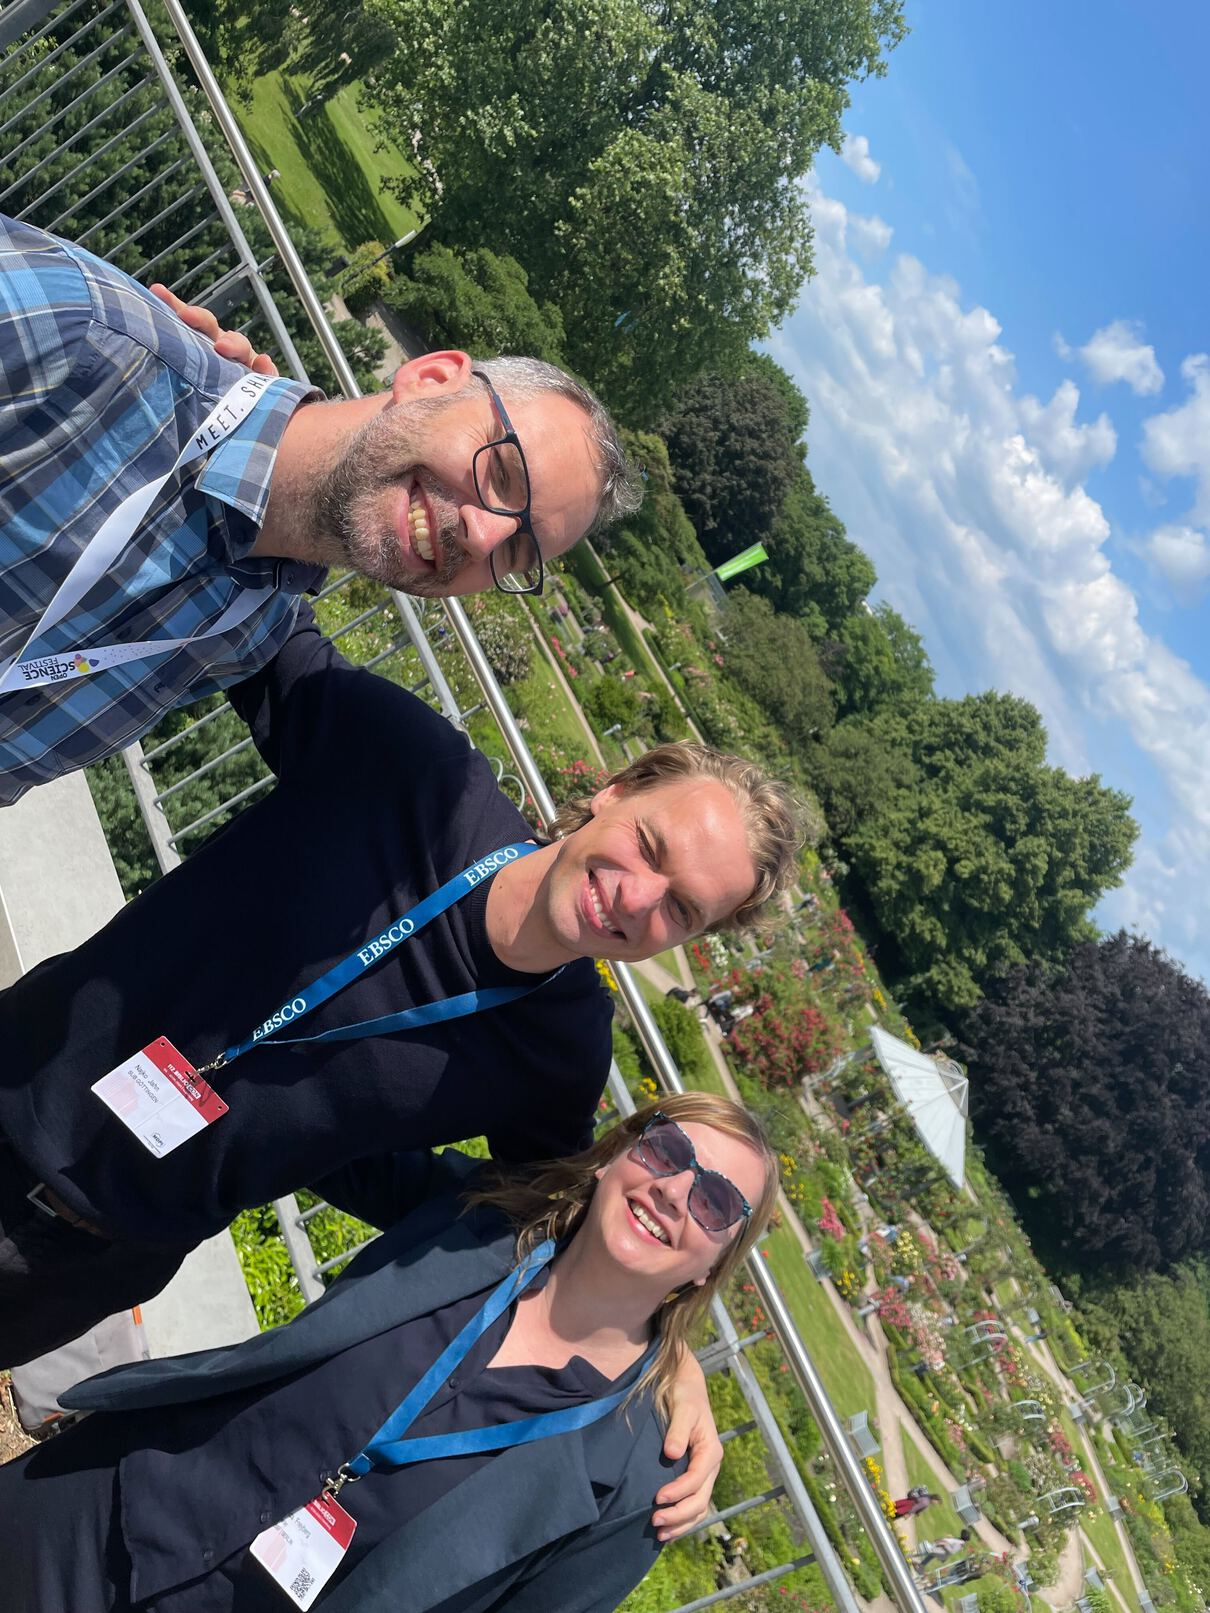
\includegraphics{image.jpg}
\caption{Abb. 1: Redaktionsorte XXIV: Hamburg, Frühling 2024}
\end{figure}

***

Zu der Zeit, in der wir für diese Ausgabe Korrektur lasen, erreichte uns
die traurige Nachricht, dass Gabriele Beger, zuletzt Direktorin der
Staats- und Universitätsbibliothek Hamburg, aber auch Lehrbeauftragte an
der Humboldt-Universität zu Berlin und Honorarprofessorin an der
Fachhochschule Potsdam, verstorben ist.

Eine ganze Anzahl von Redaktionsmitgliedern der LIBREAS studierte bei
ihr die Grundlagen des Bibliotheksrechts und hatte auch später mit ihr
immer neu motivierende Kontakte. Sie vermittelte uns dabei nicht nur,
dass dieses Thema relevant ist und interessant sein konnte, sondern sie
lebte auch eine Begeisterung für rechtliche Fragen, für Open Access und
das Bibliothekswesen im Allgemeinen vor, das sonst selten zu finden ist.

Eine ganze Anzahl von Kolleg*innen und Einrichtungen hat Nachrufe auf
Gabriele Beger veröffentlicht, was zeigt, wie geschätzt sie
war.\footnote{Unter anderem Nikolaus Bernau würdigte sie in einem
  schönen Nachruf im Tagesspiegel:
  \url{https://www.tagesspiegel.de/kultur/nachruf-auf-gabriele-beger-fechterin-fur-die-bibliotheken-und-juristin-aus-leidenschaft-11685581.html}.}
Uns bleibt diesen nichts hinzuzufügen, ausser, dass mit ihr eine Person
verstorben ist, die einiges dafür getan hat, dass wir selber im
Bibliothekswesen aktiv sind.

Ihre / eure Redaktion LIBREAS. Library Ideas

(Berlin, Brandenburg an der Havel, Göttingen, Lausanne, München)

%autor

\end{document}